\section{Information theory quantifiers}\label{sec:quanti}

Dynamical systems are systems that evolve in time.
In practice, one may only be able to measure a scalar time series ${\mathcal X}(t)$ which may be a function of variables ${\mathcal V}=\{ v_1,  v_2,\cdots, v_k\}$ describing the underlying dynamics (i.e. $d{\mathcal V}/dt=f({\mathcal V})$.
Given a time series or other observational data, we try to infer  properties of an unfamiliar system from  the analysis of measured time record of it behavior (time series).  
how much information are these data revealing about the dynamics of the underlying system or processes?
The information content of a system is typically evaluated via a probability distribution function (PDF) $P$ describing the apportionment of some measurable or observable quantity, generally a time series ${\mathcal X}(t)$. 
We can define Information Theory quantifiers as measures able to characterize relevant properties of the PDF associated with these time series, and in this way we should judiciously extract information on the dynamical system under study.
These quantifiers represent metrics on the space of PDFs for data sets, allowing to compare different sets and classifying them according to the properties of underlying processes - broadly, stochastic vs.  deterministic.

In our case, we are interested in chaotic dynamics.
Thus we are interested in metrics which take the temporal both order of observations explicitly into account; i.e. the approach is fundamentally \textit{causal} and \textit{statistical} in nature.
In a purely statistical approach, correlations between successive values from the time series are ignored or simply destroyed via construction of the PDF; while a causal approach focuses on the PDFs of data sequences.

The quantifiers selected are based on symbolic counting and ordinal pattern statistics.
For an application of alternative quantifiers based on Symbolic Dynamics to environmental data, we refer to \cite{Hauhs2008}.
The metrics to be used can be broadly classified along two categories: those which quantify the \textit{information content} of data versus those related to their \textit{complexity}.
Note that we are referring to the space of probability density functions here, not physical space.
For the sake of clarity and simplicity, we only introduce Information Theory quantifiers that are defined on discrete PDFs in this section, since we are only dealing with discrete data (time series).
However, all the quantifiers also have definitions for the continuous case \cite{Shannon1948,Frieden2004} . 

\subsection{Shannon entropy and statistical complexity}

Entropy is a basic quantity that can be regarded to as a measure of the uncertainty associated (information) to the physical process described by $P$.
When dealing with information content, the Shannon entropy is often considered as the foundational and most natural one \cite{Shannon1948,Weaver1949}.
Regarded as a measure of uncertainty, is the most paradigmatic example of these information quantifiers.

Let a $P=\{p_i; i=1,\ldots, N\}$ with $\sum_{i=1}^N p_i = 1$, be a  discrete probability distribution, with $N$ the number of possible states of the system under study.
The Shannon's logarithmic information measure reads
\begin{equation}
\label{Shannon-disc}
{\mathrm S}[P] ~=~ -\sum_{i=1}^{N} p_i \ln \left[ p_i \right] \ .
\end{equation}

If ${\mathrm S}[P] = {\mathrm S}_{\min} = 0$, we are in position to predict with complete certainty which of the possible outcomes $i$, whose probabilities are given by $p_i$, will actually take place. 
Our knowledge of the underlying process described by the probability distribution is maximal in this instance. 
In contrast, our knowledge is minimal for a uniform distribution $P_e = \{ p_i = 1/N, \forall i=1, \ldots , N \}$ since every outcome exhibits the same probability of occurrence, and the uncertainty is maximal, i.e., ${\mathrm S}[P_e] = {\mathrm S}_{\max} = \ln N$.
These two situations are extreme cases, therefore we focus on the `normalized' Shannon entropy, $0 \leq {\mathcal H} \leq 1$, given as
\begin{equation}
\label{shannon-disc-normalizada}
{\mathcal H} [P]~=~{\mathrm S}[P]  / {\mathrm S}_{\max} \ .
\end{equation}

Contrary to information content, there is no universally accepted definition of complexity. Here, we focus on describing the \textit{complexity of time series} and do not refer to the complexity of the underlying \textit{systems}.
A complex system does not necessarily generate a complex output.
In fact, “simple” models might generate complex data, while “complicated” systems might produce output data of low complexity \cite{Kantz1998}.


An intuitive notion of a quantitative complexity attributes low values both to perfectly ordered data (i.e. with vanishing Shannon entropy) as well as to uncorrelated random data (with maximal Shannon entropy.
For example, the statistical complexity of a simple oscillation or trend (ordered), but also of uncorrelated white noise (unordered) would be classified as low.
Between the two cases of minimal and maximal entropy, data are more difficult to characterize and hence the complexity should be higher.
We seek some functional ${\mathcal C} [P]$ quantifying structures present in the data which deviate from these two cases.
These structures relate to organization, correlational structure, memory, regularity, symmetry, patterns, and other properties \cite{Feldman2008}.


AAA

-----------------------------------



One suitable way to guarantee the desired properties for a complexity measure is to build the product of a measure of information and a measure of
disequilibrium, i.e. some kind of distance from the uniform (`equilibrium') distribution of the accessible states of 
a system. In this respect, \cite{Lamberti2004} an effective {\it Statistical Complexity Measure\/} (SCM) ${\mathcal C}$ was introduced, that is able to detect and discern basic dynamical properties of datasets.

Based on the seminal notion advanced by Lopez-Ruiz {\it et al.\/} \cite{LMC1995}, this statistical complexity 
measure\cite{Martin2003,Lamberti2004} is defined through the functional product form
\begin{equation}
{\mathcal C}[P] ~=~ {\mathcal Q}_{J}[P,P_e] \cdot {\mathcal H}[P]
\label{complexity}
\end{equation}
of the normalized Shannon entropy ${\mathcal H}$, see Eq.~\eqref{shannon-disc-normalizada}, and the disequilibrium 
${\mathcal Q}_{J}[ P, P_e]$ defined in terms of the Jensen-Shannon divergence ${\mathcal J}[ P, P_e]$.
The latter is given by
\begin{equation}
\label{disequilibrium}
{\mathcal Q}_{J} [ P, P_e] ~=~ Q_{0} {\mathcal J}[ P, P_e] ~=~ 
Q_{0} \{ {\mathrm S}[(P + P_e)/2 ] - {\mathrm S}[ P ]/2 - {\mathrm S}[P_e]/2\},
\end{equation}
where $Q_0$ is a normalization constant chosen 
such that $0 \leq {\mathcal Q}_{J} \leq 1$:
\begin{equation}
Q_0 ~=~ -2 \left\{  {\frac{N+1}{N}}  \ln (N+1) - \ln (2N)  +  \ln N \right\}^{-1} \ ,
\label{q0-jensen-1}
\end{equation}
The inverse of this value is obtained for the non-normalized Jensen-Shannon divergence when one of the components of $P$, say $p_m$, is equal to one and the remaining $p_j$'s are zero.

The Jensen-Shannon divergence quantifies the difference between probability distributions and 
is especially useful to compare the symbolic composition of different sequences\cite{Grosse2002}.
Note that the above introduced Information Theory quantifier depends on two different probability distributions: one associated with the system under analysis, $P$, and the other the uniform distribution $P_e$. For the latter, other reference distributions can be chosen to test whether an observed distribution is close to a target distribution.
It has been shown that there are \textit{limit curves} for complexity: for a given value of ${\mathcal H}$ and any data set, the possible ${\mathcal C}$ 
values vary between a minimum ${\mathcal C}_{min}({\mathcal H})$ and a maximum ${\mathcal C}_{max}({\mathcal H})$, 
restricting the possible values of the complexity measure \cite{Martin2006}.

----------------------------------------

BBB

----------------------------------------



One would like to assume that the degree of correlational structures would be adequately captured
by some functional ${\mathcal C} [P]$ in the same way that Shannon's entropy ${\mathrm S}[P]$ 
\cite{Shannon1948} ``captures" randomness.

Clearly, the ordinal structures present in a process is not quantified by randomness measures, 
and consequently, measures of statistical or structural complexity are necessary for a better understanding 
(characterization) of the system dynamics represented by their time series \cite{Crutchfield1998}. 
The opposite extremes of perfect order and maximal randomness are very simple to describe, because they do 
not have any structure. 
The complexity should be zero in these cases. 
At a given distance from these extremes, a wide range of possible ordinal structures exists. 
Complexity can be characterized by a certain degree of organization, structure, memory, regularity, symmetry, 
and patterns \cite{Feldman2008}. 
The complexity measure does much more than satisfy the boundary conditions of vanishing in the high- and 
low-entropy limits. 
In particular the maximum complexity occurs in the region between the system's perfectly ordered state and 
the perfectly disordered one. 
Complexity is allows us to detect essential details of the dynamics, and more importantly to characterize 
the correlational structure of the orderings present in the time series.

The perfect crystal and the isolated ideal gas are two typical examples of systems with minimum and 
maximum entropy, respectively. 
However, they are also examples of simple models and therefore of systems with zero complexity, as the
structure of the perfect crystal is completely described by minimal information (i.e., distances and 
symmetries that define the elementary cell) and the probability distribution for the accessible states 
is centered around a prevailing state of perfect symmetry. 
On the other hand, all the accessible states of the ideal gas occur with the same probability and can be
described by a ``simple" uniform distribution. 

Statistical complexity is often characterized by the paradoxical situation of a complicated dynamics 
generated from relatively simple systems. 
Obviously, if the system itself is already involved enough and is constituted by many different parts, 
it clearly may support a rather intricate dynamics, but perhaps without the emergence of typical 
characteristic patterns \cite{Kantz1998}. 
Therefore, a complex system does not necessarily generate a complex output. 
Statistical complexity is therefore related to patterned structures hidden in the dynamics,
emerging from a system which itself can be much simpler than the dynamics it generates \cite{Kantz1998}.

According to L\'opez-Ruiz, Mancini and Calbet \cite{LMC1995}, and using an oxymoron, an object, a procedure, 
or system is said to be complex when it does not exhibit patterns regarded as simple. 
It follows that a suitable complexity measure should vanish both for completely ordered and for completely 
random systems and cannot only rely on the concept of information (which is maximal and minimal for the 
above mentioned systems).
A suitable measure of complexity can be defined as the product of a measure of information and a measure of
disequilibrium, i.e. some kind of distance from the equiprobable distribution of the accessible states of 
a system. 
In this respect, Rosso and coworkers \cite{Lamberti2004} introduced an effective {\it Statistical Complexity 
	Measure\/} (SCM) ${\mathcal C}$, that is able to detect essential details of the dynamical processes 
underlying the dataset.

Based on the seminal notion advanced by L\'opez-Ruiz {\it et al.} \cite{LMC1995}, this statistical complexity 
measure\cite{Martin2003,Lamberti2004} is defined through the functional product form
\begin{equation}
{\mathcal C}[P] ~=~ {\mathcal Q}_{J}[P,P_e] \cdot {\mathcal H}[P]
\label{complexity}
\end{equation}
of the normalized Shannon entropy ${\mathcal H}$, see Eq.~\eqref{shannon-disc-normalizada}, and the disequilibrium 
${\mathcal Q}_{J}$ defined in terms of the Jensen-Shannon divergence ${\mathcal J}[ P, P_e]$.
That is,
\begin{equation}
\label{disequilibrium}
{\mathcal Q}_{J} [ P, P_e] ~=~ Q_{0} {\mathcal J}[ P, P_e] ~=~ 
Q_{0} \{ {\mathrm S}[(P + P_e)/2 ] - {\mathrm S}[ P ]/2 - {\mathrm S}[P_e]/2\},
\end{equation}
the above-mentioned Jensen-Shannon divergence and $Q_0$, a normalization constant 
such that $0 \leq {\mathcal Q}_{J} \leq 1$:
\begin{equation}
Q_0 ~=~ -2 \left\{  {\frac{N+1}{N}}  \ln (N+1) - \ln (2N)  +  \ln N \right\}^{-1} \ ,
\label{q0-jensen-1}
\end{equation}
are equal to the inverse of the maximum possible value of ${\mathcal J} [P,P_e]$.
This value is obtained when one of the components of $P$, say $p_m$, is equal to one and the remaining $p_j$ 
are zero.

The Jensen-Shannon divergence, which quantifies the difference between probability distributions, 
is especially useful to compare the symbolic composition between different sequences\cite{JS-Div1991,Grosse2002,JS-Div2014}.
Note that the above introduced SCM depends on two different probability distributions: one associated with the 
system under analysis, $P$, and the other the uniform distribution, $P_e$.
Furthermore, it was shown that for a given value of ${\mathcal H}$, the range of possible ${\mathcal C}$ 
values varies between a minimum ${\mathcal C}_{min}$ and a maximum ${\mathcal C}_{max}$, 
restricting the possible values of the SCM \cite{Martin2006}.
Thus, it is clear that important additional information related to the correlational structure between the 
components of the physical system is provided by evaluating the statistical complexity measure. 
%%%%%%%%%%%%%%%%%%%%%%%%%%%%%%%%%%%%%%%%%%%%%%%%%%%%%%%%%%%%%%%%%%%%%%%%%%%%%%%%%%%%%%%%%%%%%%%%%%%%%%%%%%%%
%In this way, the information plane ${\mathcal H} \times {\mathcal C}$ constitute a nice tool to visualizate 
%and characterize different dynamical systems.
%%%%%%%%%%%%%%%%%%%%%%%%%%%%%%%%%%%%%%%%%%%%%%%%%%%%%%%%%%%%%%%%%%%%%%%%%%%%%%%%%%%%%%%%%%%%%%%%%%%%%%%%%%%%

If our system, with associated discrete PDF, lies in a very ordered state, will be represented
by an extremely narrow PDF, that is almost all the 
$p_{i}$--values are almost zero except for a particular state $k \neq i$ with $p_{k} \cong 1$,then both
the normalized Shannon entropy and statistical complexity are close to zero (${\mathcal H} \approx 0$ and 
${\mathcal C} \approx 0$)

On the other hand, when the system under study is represented by  a very disordered state, that is when all the 
$p_{i}$--values oscillate around the same value, we have ${\mathcal H} \approx 1$ while 
${\mathcal C} \approx 0$

This point was extensively discussed by Rosso and co-workers \cite{Olivares2012A,Olivares2012B}.
The summands can be regarded to as a kind of ``distance" between  two contiguous probabilities.
Thus, a different ordering of the pertinent summands would lead to a different FIM-value, hereby its local nature.
In the present work, we follow the Lehmer lexicographic order \cite{Lehmer} in the generation of Bandt and Pompe 
PDF (see next section).

YOOOOO

The entropy $H[P]$ is the normalized version of the Entropy proposed by Shannon \cite{Shannon1948}:%
%
\begin{equation}\label{eq:sha}
H[P] = S[P] /S_{max},
\end{equation}

\noindent where $S[P]=-\sum _{j=1}^{M}~p_j~\ln( p_j )$ and $S_{max}$ is the normalizing constant:%
%
\begin{equation}
\label{eq:Smax} S_{max}= S[P_e] = \ln M,
\end{equation}

\noindent and $P_e=\{ 1/M, \dots,1/M\}$ is the uniform distribution.

The statistical complexity $C[P]$ is given by:
\begin{equation}
\label{eq:inten}
C[{P}]=Q_{J}[{P,P_e}]\cdot H[{P}] \ ,
\end{equation}
, and
$Q_{J}$ is named disequilibrium and it is the distance between $P$ and $P_e$ in the probability space.
The metric used in this paper is based on the Jensen-Shannon divergence \cite{Lamberti2004}:%
%
\begin{equation}
\label{eq:disequi}
Q_{J}[{P,P_e}]= Q_0 \cdot \{S[\frac{P+P_e}{2}]-S[P]/2-S[P_e]/2 \} \ .
\end{equation}
%
\noindent The normalization constant $Q_0$ is:
\begin{equation}
\label{eq:q0j}
Q_0=-2 \left\{ \left( \frac{N+1}{N} \right) \ln(N+1) - 2 \ln(2N) + \ln N \right\}^{-1} .
\end{equation}

From the statistical point of view the disequilibrium $Q_J$ is an intensive magnitude, and it is $0$ if and only if $P=P_e$.
It has been proved that the $C[P]$ quantifies the presence of nonlinear correlations typical of chaotic systems \cite{Martin2003,Lamberti2004}.
The complexity $C[P]$ is independent from the entropy $H[P]$, as far as different $P$'s share the same entropy $H[P]$ but they have different complexity $C[P]$.

\subsection{Determination of a probability distribution}

AAA

The quantifiers from Information Theory rely on a probability distribution associated to the time series. 
The determination of the most adequate PDF is a fundamental problem because the PDF $P$ and its sample space 
$\Omega$ are inextricably linked. The usual histogram technique is inadequate since the data are treated purely stochastic and the temporal information is completely lost. 
However, Bandt and Pompe (BP)\cite{Bandt2002} introduced a simple and robust symbolic methodology that takes into account time ordering of the time series by comparing neighboring values in a time series.
The symbolic data are:
{\it (i)\/}~created by ranking the values of the series; and
{\it (ii)\/}~defined by reordering the embedded data in ascending order, which is tantamount to a phase space 
reconstruction with embedding dimension (pattern length) $D$ and time lag $\tau$ (see Information for a more detailed description). 
In this way, it is possible to quantify the diversity of the ordering symbols (patterns) derived from a scalar 
time series.
Note that the appropriate symbol sequence arises naturally from the time series, and no model-based assumptions 
are needed.
As such, it allows to uncover important details concerning the ordinal structure of the time series
\cite{Rosso2007} and can also yield information about temporal correlation \cite{Rosso2009}.

This type of analysis of a time series entails losing details of the original series' amplitude information. However, the symbolic representation of time series by recourse to a comparison of consecutive ($\tau = 1$) or nonconsecutive ($\tau > 1$) values allows for an accurate empirical reconstruction of the underlying phase-space, even in the presence of weak (observational and dynamic) noise \cite{Bandt2002}. Furthermore, the ordinal patterns associated with the PDF are invariant with respect to nonlinear monotonous transformations; nonlinear drifts or scaling artificially introduced by a measurement device will not modify the estimation of quantifiers, a nice property if one deals with experimental data (see, e.g., \cite{Saco2010}. 
The only condition for the applicability of the BP method is a very weak stationary assumption: for 
$k \leq D$, the probability for $x_t < x_{t+k}$ should not depend on $t$.
For a review of BP's methodology and its applications to physics, biomedical and econophysics signals, see \cite{Zanin2012}. 

Regarding the selection of the parameters, Bandt and Pompe suggested working with $4 \leq D \leq 6$ for typical time series lengths, and specifically considered a time lag $\tau = 1$ in their cornerstone paper \cite{Bandt2002}.For the artificially generated time series shown below(Figs 1 and 2),we chose D= 6 and follow the Lehmer-permutation scheme [35] to calculate the Fisher Information. For themeasured andmodelled time series analyzed here, the embedding dimension is chosen as D= 4 throughout due to time series length requirements (S1 File), in particular at coarse tem- poral resolution, and to achieve comparability across the different analyses. In all cases, the delay parameter has been set to tau = 1.

Incorporating amplitude information: Weighted ordinal pattern distribution:
Recently, the permutation entropy was extended to incorporate also amplitude information [40].Hence, a potential disadvantage of ordinal pattern statistics, namely the loss of amplitude information, can be addressed by introducingweights in order to obtain a ‘weighted permuta- tion entropy (WPE)’. In the context of environmental time series,which typically exhibit a pro- nounced seasonal cycle and thus seasonally varying signal to noise ratios, this ideamight be particularly useful to address (noisy) low-variance patterns (e.g. during dormancy periods in winter). Weighting the probabilities of individual patterns according to their variance alleviates
potential issues regarding to ‘high noise, low signal’ patterns, because low-variance patterns that are stronlgy affected by noise are down-weighted in the resulting ‘weighted ordinal pattern distributions’. For example, [40] show that a weighted entropymeasure is sensitive to sudden changes in the variance of the time series.Here, we extend the idea ofWPE following [40] to derive a weighted permutation entropy (Hw
), weighted statistical complexity (Cw ), and
weighted Fisher Information (Fw
).
Non-normalizedweights are computed for each temporalwindowfor the time seriesX, such that
X
D wj Here, the embedding dimension is denoted by D and XD j denotes the arithmeticmean of the
time series in the currentwindowwith index j. Thus, theweight of each windowof lengthDis given by its variance in the equation above. The weights wj are then used tomodify the relative frequencies of each ordinal pattern pj

The denominator of this equation provides the normalization, and the Kronecker delta fasd
in the enumerator serves to indicatewhich pattern occurs in each windowj:
(1;
if piasdf pj
;
dpi;pj
asdf 0;
if pi
6fasd pj
:
After having calculated the appropriate asdfi for each i = 1, . . .,D!, the same Eqs (2), (3) and (6) are applied to obtain the weighted versionsHw
, Cw and Fw of the ITQ. The weighting of the ITQcan be considered as noise filter, provided that noise is character-
ized by relatively low variance, and thus enhances the signal contained in the time series. In any case, rare patterns are suppressed in favour ofmore frequent ones. Obviously, the window-basedvariance is but one out ofmany weighting recipes, others are
easily conceivable. There is also a connection to the celebrated Rènyi entropy ([41])
!
X
D!
Hq
asdfXSS asdf 1 1 ? q log2
pq i
ifds1
where the Rènyi exponent q suppresses low-frequency patterns for q>1; for q = 1, the Shan- non entropy is obtained. The resulting ‘Rènyi ordinal pattern distribution’ could be considered as a special case of the weighted pattern distribution, characterized by a single exponent; this has not been investigated so far, however. Summarizing, ITQcomputed based on an appropriately weighted formof the ordinal pat-
tern distribution are suitable to analyse data setswith considerable amplitude information (e.g. seasonal variation) froman information-theoretic viewpoint. Since this is an issue for the time series investigated here, we willmostly performour ITQanalysis using theweighted versions describedhere.

BBB

The evaluation of the Information Theory derived quantifiers, like those previously introduced (Shannon entropy,
Fisher information and statistical complexity), suppose some prior knowledge about the system; specifically, 
a probability distribution associated to the time series under analysis should be provided beforehand. 
The determination of the most adequate PDF is a fundamental problem because the PDF $P$ and the sample space 
$\Omega$ are inextricably linked. 

Usual methodologies assign to each time point of the series ${\mathcal X}(t)$ a symbol from a  finite alphabet 
$\mathcal{A}$, thus creating a {\it symbolic sequence} that can be regarded to as a {\it non causal coarse 
	grained\/} description of the time series under consideration. 
As a consequence, order relations and the time scales of the dynamics are lost. 
The usual histogram technique corresponds to this kind of assignment.
{\it Causal information\/}  may be duly incorporated if information about the past dynamics of the system is 
included in the symbolic sequence, i.e., symbols of alphabet $\mathcal{A}$ are assigned to a portion of the 
phase-space or trajectory.

Many methods have been proposed for a proper selection of the probability space $(\Omega, P)$. 
Among others, of type non causal coarse grained, we can mention frequency counting \cite{Rosso2009C}, 
procedures based on amplitude statistics \cite{DeMicco2008}, binary symbolic dynamics \cite{Mischaikow1999},
Fourier analysis \cite{Powell1979}, or wavelet transform \cite{Rosso2001}. 
The suitability of each of the proposed methodologies depends on the peculiarity of data, such as stationarity, 
length of the series, the variation of the parameters, the level of noise contamination, etc. 
In all these cases, global aspects of the dynamics can be somehow captured, but the different approaches 
are not equivalent in their ability to discern all relevant physical details.
Bandt and Pompe (BP)\cite{Bandt2002} introduced a simple and robust symbolic methodology that takes into account 
time causality of the time series (causal coarse grained methodology) by comparing neighboring values in a 
time series.
The symbolic data are:
{\it (i)\/}~created by ranking the values of the series; and
{\it (ii)\/}~defined by reordering the embedded data in ascending order, which is tantamount to a phase space 
reconstruction with embedding dimension (pattern length) $D$ and time lag $\tau$.
In this way, it is possible to quantify the diversity of the ordering symbols (patterns) derived from a scalar 
time series.

Note that the appropriate symbol sequence arises naturally from the time series, and no model-based assumptions 
are needed.
In fact, the necessary ``partitions'' are devised by comparing the order of neighboring relative values rather 
than by apportioning amplitudes according to different levels.
This technique, as opposed to most of those in current practice, takes into account the temporal structure of 
the time series generated by the physical process under study.
As such, it allows us to uncover important details concerning the ordinal structure of the time series
\cite{Rosso2007,Rosso2012A,Rosso2012B,Rosso2013} and can also yield information about temporal correlation 
\cite{Rosso2009A,Rosso2009B}.

It is clear that this type of analysis of a time series entails losing details of the original series' 
amplitude information.
Nevertheless, by just referring to the series' intrinsic structure, a meaningful difficulty reduction has 
indeed been achieved by BP with regard to the description of complex systems.
The symbolic representation of time series by recourse to a comparison of consecutive ($\tau = 1$) or 
nonconsecutive ($\tau > 1$) values allows for an accurate empirical reconstruction of the underlying phase-space, 
even in the presence of weak (observational and dynamic) noise \cite{Bandt2002}.
Furthermore, the ordinal patterns associated with the PDF are invariant with respect to nonlinear monotonous 
transformations.
Accordingly, nonlinear drifts or scaling artificially introduced by a measurement device will not modify the 
estimation of quantifiers, a nice property if one deals with experimental data (see, e.g., \cite{Saco2010}).
These advantages make the BP methodology more convenient than conventional methods based on range 
partitioning, i.e., a PDF based on histograms.

To use the BP methodology\cite{Bandt2002} for evaluating the PDF, $P$, associated with the time 
series (dynamical system) under study, one starts by considering partitions of the $D$-dimensional space that 
will hopefully ``reveal'' relevant details of the ordinal structure of a given one-dimensional time series 
${\mathcal X}(t) = \{ x_t; t = 1, \ldots, M\}$ with embedding dimension $D > 1$ ($D \in {\mathcal N}$) 
and time lag $\tau$ ($\tau \in {\mathcal N}$).
We are interested in ``ordinal patterns'' of order (length) $D$ generated by
\begin{equation}
\label{asignation1}
(s)\mapsto \left(x_{s-(D-1)\tau},x_{s-(D-2)\tau},\ldots, x_{s-\tau},x_{s}\right) \ ,
\end{equation}
which assign to each time $s$ the $D$-dimensional vector of values at times $s-(D-1)\tau,\ldots,s-\tau,s$.
Clearly, the greater $D$, the more information on the past is incorporated into our vectors.
By ``ordinal pattern'' related to the time $(s)$, we mean the permutation $\pi=(r_0,r_1, \ldots,r_{D-1})$ 
of $[0,1,\ldots,D-1]$ defined by 
\begin{equation}
\label{asignation2}
x_{s-r_{D-1}\tau} \le~x_{s-r_{D-2}\tau} \le \cdots \le~x_{s-r_{1}\tau} \le x_{s-r_0\tau}  .
\end{equation}
In this way the vector defined by Eq. (\ref{asignation1}) is converted into a unique symbol $\pi$.
We set $r_i < r_{i-1}$ if $x_{s-r_{i}} = x_{s-r_{i-1}}$ for uniqueness, although ties in samples from 
continuous distributions have null probability.

In order to illustrate BP method, we will consider  a simple example: a time series with seven 
($M=7$) values ${\mathcal X} = \{4, 7, 9, 10, 6, 11, 3\}$ and we evaluate the BP-PDF for $D=3$ and $\tau=1$.
In this case the state space is divided into $3!$ partitions and $6$ mutually exclusive permutation symbols 
are considered.
The triplet $(4, 7, 9)$ and $(7, 9, 10)$ represent the permutation pattern $[012]$ since they are in 
increasing order.
On the other hand, $(9, 10, 6)$ and $(6, 11, 3)$ correspond to the permutation pattern $[201]$ since 
$x_{s+2} < x_s < x_{s+1}$, while $(10, 6, 11)$ has the permutation pattern  $[102]$ with 
$x_{s+1} < x_s < x_{s+2}$.
Then, the associated probabilities to the $6$ patterns are:
$p([012]) = p([201]) = 2/5$; $p([102]) = 1/5$; $p([021]) = p([120]) = p([210])=0$.

Figure~\ref{fig:patrones} illustrates the construction principle of the ordinal patterns of length 
$D=2$, $3$ and $4$ with $\tau = 1$\cite{Parlitz2012}.
Consider the sequence of observations $\{x_0, x_1, x_2, x_3\}$.
For $D=2$, there are only two possible directions from $x_0$ to $x_1$: up and down.
For $D=3$, starting from $x_1$ (up) the third part of the pattern can be above $x_1$, below $x_0$, or between 
$x_0$ and $x_1$.
A similar situation can be found starting from $x_1$ (down). 
For $D=4$, for each one of the six possible positions for $x_2$, there are four possible localizations for $x_3$, 
yielding $D!=4!=24$ different possible ordinal patterns.
In Fig.~\ref{fig:patrones}, full circles and continuous lines represent the sequence values 
$x_0 < x_1 > x_2 > x_3$, which leads to the pattern  $\pi=[0321]$.
A graphical representation of all possible patterns corresponding to $D = 3, 4$ and $5$
can be found in Fig.~2 of Parlitz \textit{et al.}\cite{Parlitz2012}.


For all the $D!$ possible orderings (permutations) $\pi_i$ when  embedding dimension is $D$, 
and time-lag $\tau$,
their relative 
frequencies can be naturally computed according to the number of times this particular order sequence is found 
in the time series,  divided by the total number of sequences,
\begin{equation}
\label{eq:frequ}
p(\pi_i)= \frac{\# \{s|s\leq N-(D-1)\tau ; (s)  \text{ is of type } \pi_i \}}{N-(D-1)\tau} ,
\end{equation}
where $\#$ denotes cardinality.
Thus, an ordinal pattern probability distribution $P = \{ p(\pi_i), i = 1, \dots, D! \}$ is obtained from the 
time series.

The embedding dimension $D$ plays an important role in the evaluation of the appropriate probability 
distribution, because $D$ determines the number of accessible states $D!$ and also conditions the minimum 
acceptable length $M \gg D!$ of the time series that one needs in order to work with reliable statistics 
\cite{Kowalski2007}.
In the present work, we follow the Lehmer lexicographic order \cite{Lehmer} in the generation of Bandt and 
Pompe PDF.

Regarding the selection of the parameters, Bandt and Pompe suggested working with $4 \leq D \leq 6$, and 
specifically considered a time lag $\tau = 1$ in their cornerstone paper \cite{Bandt2002}.
Nevertheless, it is clear that other values of $\tau$ could provide additional information.
It has been recently shown that this parameter is strongly related, if it is relevant, to the intrinsic 
time scales of the system under analysis \cite{Zunino2010B,Soriano2011,Zunino2012}.

Additional advantages of the  method reside in
{\it i)\/} its simplicity (it requires few parameters: the pattern length/embedding dimension $D$ and the 
time lag $\tau$), and
{\it ii)\/} the extremely fast nature of the calculation process. %\cite{Keller2005}.
The BP methodology can be applied not only  to time series representative of low dimensional dynamical 
systems, but also to any type of time series (regular, chaotic, noisy, or reality based).
In fact, the existence of an attractor in the $D$-dimensional phase space in not assumed.
The only condition for the applicability of the BP method is  a very weak stationary assumption: for 
$k \leq D$, the probability for $x_t < x_{t+k}$ should not depend on $t$.
For a review of BP's methodology and its applications to physics, biomedical and econophysics signals see 
Zanin {\it et al.\/} \cite{Zanin2012}. 
Moreover, Rosso {\it et al.\/} \cite{Rosso2007} show that the above mentioned quantifiers produce better 
descriptions of the process associated dynamics when the PDF is computed using BP rather than using the 
usual histogram methodology.

The BP proposal for associating probability distributions to time series (of an underlying symbolic 
nature) constitutes a significant advance in the study of nonlinear dynamical systems \cite{Bandt2002}.
The method provides univocal prescription for ordinary, global entropic quantifiers of the Shannon-kind.
However, as was shown by Rosso and coworkers \cite{Olivares2012A,Olivares2012B}, ambiguities arise in 
applying the BP technique with reference to the permutation of ordinal patterns. 
This happens if one wishes to employ the BP-probability density to construct local entropic quantifiers, 
like the Fisher information measure, which would characterize time series generated by nonlinear dynamical 
systems.

The local sensitivity of the Fisher information measure for discrete PDFs is reflected in the fact that the 
specific ``$i$-ordering'' of the discrete values $p_i$ must be seriously taken into account in evaluating 
Eq.~(\ref{Fisher-disc}).
The numerator can be regarded to as a kind of ``distance'' between two contiguous probabilities.
Thus, a different ordering of the summands will lead, in most cases, to a different Fisher information value.
In fact, if we have a discrete PDF given by $P = \{ p_i, i = 1, \ldots , N\}$, we will have $N!$ possibilities 
{for the $i$-ordering.}

The question is, which is the arrangement that one could regard as the ``proper'' ordering?
The answer is straightforward in some cases, like the one that pertains to histogram-based PDFs. 
For extracting a time-series PDF $P$ via an histogram procedure, one first divides the interval $[a,b]$ 
(with $a$ and $b$ the minimum and maximum amplitude values in the time series) into a finite number $N_{bin}$ 
($N \equiv N_{bin}$ in Eqs. (\ref{Shannon-disc}) and (\ref{Fisher-disc})) of non overlapping equal sized 
consecutive subintervals $A_k:[a,b]=\bigcup_{k=1}^{N_{bin}} A_k$ and $A_n \bigcap A_m=\emptyset~\forall n\neq m$. 
Then, recourse to the usual histogram method, based on counting the relative frequencies of the time series'
values within each subinterval, is made. 
Of course, in this approach the temporal order in which  the time-series values emerge plays no role at all. 
The only pieces of information we have here are the $x_t$-values that allow one to assign inclusion within a 
given bin, ignoring just where they are located (this is, the subindex $i$). 
Note that the division procedure of the interval $[a, b]$ provides the natural order sequence for the evaluation
of the PDF gradient involved in Fisher's information measure.

From now on, we assume that the all Information Theory quantifiers will be evaluated with BP-PDF's,
by this reason usually they are called permutation quantifiers or time causal Information Theory quantifiers.
In our current paper, we chose the lexicographic ordering given by the algorithm of Lehmer \cite{Lehmer}, 
among other possibilities, due to its better distinction of different dynamics in the Shannon--Fisher plane, 
${\mathcal H} \times {\mathcal F}$ (see \cite{Olivares2012A,Olivares2012B}). 

YOOOO

All the statistical quantifiers studied here are functionals of the PDF associated to the time series.
The first step to quantify the statistical properties of the values (amplitude statistics) of a time series $\{x_i, \forall \; i=1,\dots,N\}$ using information theory is to determine the concomitant PDF.
This is an issue studied in detail in previous papers \cite{aka varios}.
Let us summarize the procedure:
\begin{enumerate} 
	\item \label{1} a finite alphabet with $M$ symbols $\mathcal{A}=\{a_1,\dots,a_M\}$ is chosen. 
	\item \label{2} each one of these symbols is assigned to each: (a) value of the time series (or non-overlapped set of consecutive values) or (b) portion of length $D$ of the trajectory.
	\item \label{3} the normalized histogram of the symbols is the desired PDF.
	\item \label{4} a randomness quantifier is calculated over the PDF. In our case we calculate (a) normalyzed Shannon entropy $H$, (b) normalyzed statistical complexity $C$ and (d) MP.
\end{enumerate}

Note that if option (a) is chosen in step \ref{2} then the PDF is non causal, because all the information about the time evolution of the system generating $\{x_i\}$ is completely lost.
On the contrary if option (b) is chosen in step \ref{2} then the PDF is causal, in the sense it includes information about the temporal evolution.

\textcolor{red}{NOMBRAR LA BPW}

\textcolor{red}{NOMBRAR LOS PLANOS QUE TERMINEMOS ELIGIENDO}

Of course there are infinite possibilities to choose the alphabet $\mathcal{A}$ as well as the length $D$.
Bandt \& Pompe made a proposal for a causal PDF that has been shown to be easy to implement and useful in a great variety of applications \textcolor{red}{REFERENCIAS A APLICACIONES}.
The procedure is the following \cite{Bandt2002,Keller2003,Keller2005}: \textcolor{red}{ESTA PARTE ESTÁ EN EL TIEMPO Y DEBERÍA ESTAR EN LAS MUESTRAS}

\begin{itemize}
	\item Given a series $\{x_t, \forall \;  t=0, \Delta t, \cdots,N\Delta t \}$, a sequence of vectors of length $D$ is generated.
	
	\begin{equation}
	(s)\longmapsto\left(x_{t-(d-1)\Delta t},x_{t-(d-2)\Delta t},\dots,x_{t-\Delta t},x_{t}\right) 
	\label{eq:vectores}
	\end{equation}
	\\
	Each vector turns out to be the ``history'' of the value $x_t$. Clearly, the longer the length of the vectors $D$, the more information about the history would the vectors have but a higher value of $N$ is required to have an adequate statistics. 
	\\
	\item The permutations $\pi=(r_0, r_1, \cdots, r_{D-1})$ of $(0, 1, \cdots, D-1)$ are called ``order of patterns'' of time $t$, defined by:
	
	\begin{equation}
	\label{eq:permuta}
	x_{t-r_{D-1}\Delta t}\le x_{t-r_{D-2}\Delta t}\le\dots\le x_{t-r_{1}\Delta t}\le x_{t-r_0\Delta t}
	\end{equation}
	\\
	In order to obtain an unique result it is considered $r_i<r_{i-1}$ if $x_{t-r_{i}\Delta t}=x_{t-r_{i-1}\Delta t}$.
	
	In this way, all the $D!$ possible permutations $\pi$ of order $D$, and the PDF $P=\{p(\pi)\}$ is defined as:
	
	\begin{equation}
	\label{eq:frequ}
	p(\pi)=\frac{\sharp \{s|s\leq N-D+1; (s) \quad \texttt{has type}~\pi\}}{N-D+1}
	\end{equation}
	
	In the last expression the $\sharp$ symbol means ``number".
\end{itemize}

This procedure has the advantages of being {\it i}) simple, {\it ii}) fast to calculate, {\it iii}) robust in presence of noise, and {\it iv}) invariant to lineal monotonous transformations. \textcolor{red}{DICE QUE ES ROBUSTO FRENTE A LA PRESENCIA DE RUIDO PERO NO, REFERENCIAS?}

It is applicable to weak stationarity processes (for $k=D$, the probability that $x_t < x_{t+k}$ doesn't depend on the particulary $t$ \cite{Bandt2002}).The causality property of the PDF allows the quantifiers (based on this PDFs) to discriminate between deterministic and stochastic systems \cite{Rosso2007B}.

According to this point Bandt and Pompe suggested $3\leq D \leq 7$. $D=6$ has been adopted in this work.

\subsection{Information Planes}

AAA

A particularly useful visualization of the quantifiers from Information Theory is their juxtaposition in two-dimensional graphs. Three  such \textit{causal information planes} can be defined: 
{\it a)\/} The {\it causality entropy--complexity plane\/}, ${\mathcal H} \times {\mathcal C}$, is based 
only on global characteristics of the associated time series PDF (both quantities are defined in terms of 
Shannon entropies); while 
{\it b)\/} the {\it causality Shannon-Fisher plane\/}, ${\mathcal H} \times {\mathcal F}$, is based on 
global and local characteristics of the PDF; finally, {\it c)\/} the plane spanned by ${\mathcal C} \times {\mathcal F}$ is of course fully redundant to the other two.  
In the case of ${\mathcal H} \times {\mathcal C}$ the value range is $[0, 1] \times [{\mathcal C}_{min}(\mathcal{H}), 
{\mathcal C}_{max}(\mathcal{H})]$, while in the causality 
plane ${\mathcal H} \times {\mathcal F}$ the range is presumably $[0, 1]\times [0, 1]$; no limit curves have been shown to exist so far.

These diagnostic tools were shown to be particularly efficient to distinguish between the deterministic chaotic and stochastic nature of a time series since the permutation quantifiers have distinct behaviours for different types of processes, see Figs. \ref{fig1} and \ref{fig2}, respectively. 
%For the purpose of this paper, all results for the ${\mathcal H} \times %{\mathcal F}$ plane are shown in the main text, while all results with %respect to the ${\mathcal H} \times {\mathcal C}$ plane are shown in the %Supplementary Material.

Chaotic maps have intermediate entropy ${\mathcal H}$ and Fisher ${\mathcal F}$ values, while their complexity 
${\mathcal C}$ reaches larger values, very close to those of the upper complexity limit \cite{Rosso2007,Olivares2012B}. For regular processes, entropy and complexity have small values, close to zero, while the Fisher information is close to one. 
Uncorrelated stochastic processes are located in the planar location associated with
${\mathcal H}$ near one and ${\mathcal C}$, ${\mathcal F}$ near zero, respectively.
It has also been found that correlated stochastic noise processes with a power spectrum proportional to $1/f^k$, where $1 \leq k \leq 3$, are characterized by intermediate permutation entropy and intermediate statistical complexity values \cite{Rosso2007}, as well as intermediate to low Fisher information \cite{Olivares2012B}.
In both causal information planes (${\mathcal H} \times {\mathcal C}$, see Fig. \ref{fig1} and  ${\mathcal H} \times {\mathcal F}$, see Fig. 
\ref{fig2}), stochastic data are clearly localized at different planar positions than deterministic chaotic ones. 
%%%%%%%%%OTRAS APLICACIONES-1:
These two causal information planes have been profitably used to visualize and characterize different dynamical regimes when the system parameters vary  
\cite{Olivares2012A,Olivares2012B,Rosso2010,Kowalski2011,DeMicco2012,Lange2013,Serinaldi2014,Montani2014A,Montani2014B,Montani2015A,
	Montani2015B,Aquino2015}; 
%%%%%%%%%OTRAS APLICACIONES-2:
to study temporal dynamic evolution 
\cite{Kowalski2007,Bariviera2015A,Bariviera2015B};
%%%%%%%%%OTRAS APLICACIONES-3:
to identify periodicities in natural time series 
\cite{Bandt2005};
%%%%%%%%%OTRAS APLICACIONES-4: 
to identify deterministic dynamics contaminated with noise 
\cite{Rosso2012A,Rosso2012B};
%%%%%%%%%OTRAS APLICACIONES-5: 
to estimate intrinsic time scales and delayed systems 
\cite{Zunino2010B,Soriano2011,Zunino2012};
%%%%%%%%%OTRAS APLICACIONES-6:
for the characterization of pseudo-random number generators
\cite{Demico2008,Demico2012};
%%%%%%%%%OTRAS APLICACIONES-7:
to quantify the complexity of two-dimensional patterns
\cite{Ribeiro2012}, and 
%%%%%%%%%OTRAS APLICACIONES-8:
for other biomedical and econophysics applications (see \cite{Zanin2012} and references therein).

BBB

In statistical mechanics one is often interested in isolated systems  characterized by an initial, arbitrary,
and discrete probability distribution. 
Evolution towards equilibrium is to be described, as the overriding goal.
At equilibrium, we can suppose, without loss of generality, that this state is given by the equiprobable 
distribution $P_e = \{ p_i = 1/N, \forall i=1, \ldots , N \}$.
The temporal evolution of the above introduced Information Theory quantifiers, Shannon entropy $\mathcal H$, 
statistical complexity $\mathcal C$ and Fisher information measure $\mathcal F$, can be analyzed using a 
two-dimensional (2D) diagrams of the corresponding quantifiers versus time $t$. 
However, the second law of thermodynamics states that, for isolated systems, entropy grows monotonically
with time ($d{\mathcal H}/dt \geq 0$) \cite{Plastino1996}. 
This implies that entropy ${\mathcal H}$ can be regarded as an arrow of time, so that an equivalent way
to study the temporal evolution of these quantifiers is using the normalized entropy ${\mathcal H}$ as 
substitute for the time-axis.

Two causal information planes are defined (the term causality remembers the fact that temporal correlations 
between successive samples are taken into account through the Bandt and Pompe PDF recipe used to
estimate both Information Theory quantifiers):
{\it a)\/} The {\it causality entropy--complexity plane\/}, ${\mathcal H} \times {\mathcal C}$, is based 
only on global characteristics of the associated time series PDF (both quantities are defined in terms of 
Shannon entropies); while 
{\it b)\/} the {\it causality Shannon-Fisher plane\/}, ${\mathcal H} \times {\mathcal F}$, is based on 
global and local characteristics of the PDF.
In the case of ${\mathcal H} \times {\mathcal C}$ the variation range is $[0, 1] \times [{\mathcal C}_{min}, 
{\mathcal C}_{max}]$ (with ${\mathcal C}_{min}$ and ${\mathcal C}_{max}$ the minimum and maximum statistical 
complexity values, respectively, for a given ${\mathcal H}$ value \cite{Martin2006}), while in the causality 
plane ${\mathcal H} \times {\mathcal F}$ the range is $[0, 1]\times [0, 1]$.

These two diagnostic tools were shown to be particularly efficient to distinguish between the deterministic 
chaotic and stochastic nature of a time series since the permutation quantifiers have distinctive behaviors 
for different types of motion.
According to the findings obtained by Rosso {\it et al.\/} \cite{Rosso2007,Olivares2012B,Rosso2015PP}, 
chaotic maps have intermediate entropy ${\mathcal H}$ and Fisher ${\mathcal F}$ values, while complexity 
${\mathcal C}$ reaches larger values, very close to those of the limit. 
For regular processes, entropy and complexity have small values, close to zero, while the Fisher is close
to one. 
Finally, totally uncorrelated stochastic processes are located in the planar location associated with
${\mathcal H}$ near one and, ${\mathcal C}$, ${\mathcal F}$ near to zero, respectively.
It has also been found that $1/f^\alpha$ correlated stochastic processes with $1 \leq \alpha \leq 3$ are 
characterized by intermediate permutation entropy and intermediate statistical complexity values
\cite{Rosso2007}, as well as,  intermediate low Fisher information \cite{Rosso2007,Olivares2012B,Rosso2015PP}.
Moreover, note that in both causal information planes the localization of these stochastic behavior look like 
a separation border with respect to chaotic, which are localized above of it.
%%%%%%%%%OTRAS APLICACIONES-1:
In addition, these two causal information planes have been profitably used to visualization and characterization 
of different dynamical regimes when the system parameters vary  
\cite{Olivares2012A,Olivares2012B,Rosso2010,Kowalski2011,DeMicco2012,Lange2013,Serinaldi2014,Montani2014A,Montani2014B,Montani2015A,Montani2015B}; 
%%%%%%%%%OTRAS APLICACIONES-2:
to study time dynamic evolution 
\cite{Kowalski2007,Bariviera2015A,Bariviera2015B};
%%%%%%%%%OTRAS APLICACIONES-3:
identifying periodicities in natural time series 
\cite{Bandt2005};
%%%%%%%%%OTRAS APLICACIONES-4: 
identification of deterministic dynamics contaminated with noise 
\cite{Rosso2012A,Rosso2012B};
%%%%%%%%%OTRAS APLICACIONES-5: 
estimating intrinsic time scales and delayed systems 
\cite{Zunino2010B,Soriano2011,Zunino2012,Aquino2015};
%%%%%%%%%OTRAS APLICACIONES-6:
characterization of pseudo-random number generators
\cite{Demico2008,Demico2012}
%%%%%%%%%OTRAS APLICACIONES-7:
measure of complexity of two-dimensional patterns
\cite{Ribeiro2012}
%%%%%%%%%OTRAS APLICACIONES-8:
among other biomedical and econophysics applications (see \cite{Zanin2012} and references therein).

YOOOOO

Two representation planes are considered: $H_{BP}$ vs $H_{hist}$ \cite{DeMicco2008} and $H_{BP}$ vs $C_{BP}$ \cite{Rosso2007}.
In the first plane a higher value in any of the entropies, $H_{BP}$ and $H_{hist}$, implies an increase in the uniformity of the involved PDF.
The point $(1,1)$ represents the ideal case with uniform histogram and uniform distribution of ordering patterns.
In the second plane not the entire region $0<H_{BP}<1$, $0<C_{BP}<1$ is achievable.
In fact for any PDF the pairs $(H,C)$ of possible values fall between two extreme curves in the plane $H$-$C$ \cite{Anteneodo1996}.
Fig. \ref{fig:CbpHbp} shows two regions labeled as deterministic and stochastic. In fact transition from one region to the other are smooth and the division is a bit arbitrary. 
A more detailed discussion can be seen in \cite{Rosso2007}. 
Ideal random systems having uniform Bandt \& Pompe PDF, are represented by the point $(1,0)$ \cite{Gonzalez2005} and a delta-like PDF corresponds with the point $(0,0)$.

\begin{figure}
	\centering	
	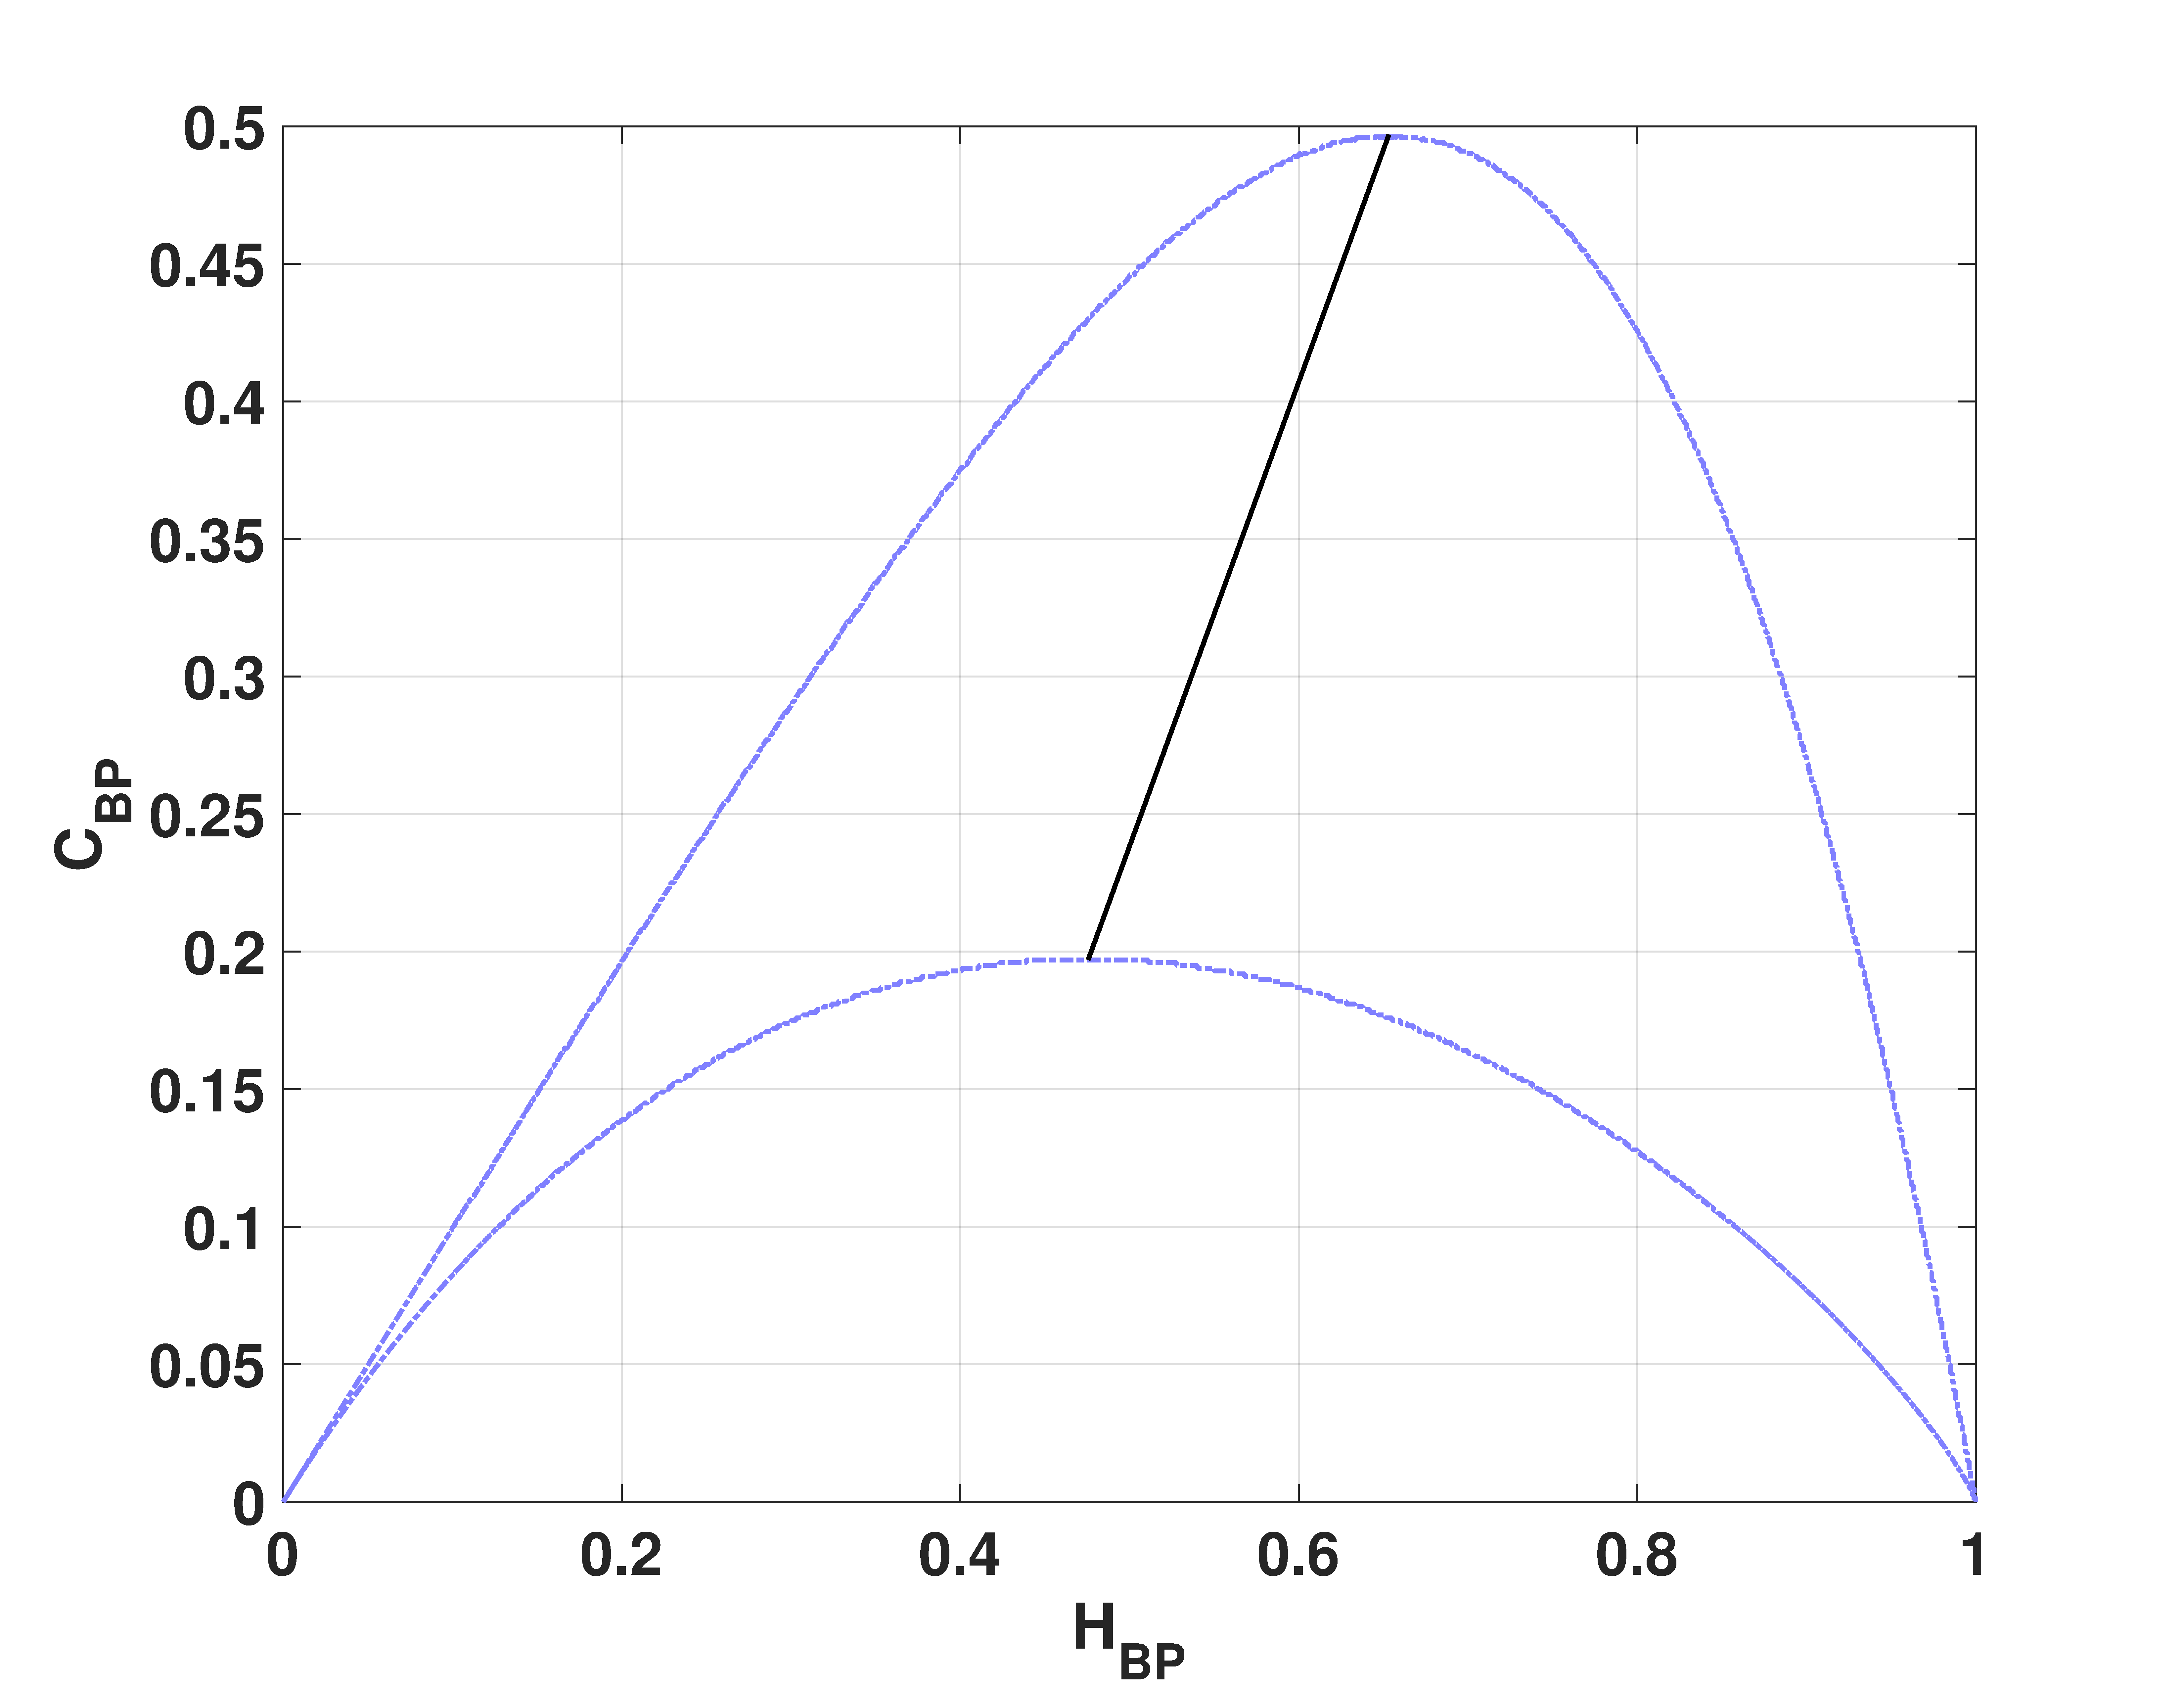
\includegraphics[width= .49\textwidth]{CbpHbp}
	\caption{Entropy-Complexity plane.}
	\label{fig:CbpHbp}
\end{figure}

We also used the number of MP as a quantifier\cite{Rosso2012}.
As shown recently by Amig\'o {\it et al.} \cite{Amigo2006,Amigo2007,Amigo2008,Amigo2010}, in the case of deterministic one-dimensional maps, not all the possible ordinal patterns can be effectively materialized into orbits, which in a sense makes these patterns forbidden.
Indeed, the existence of these forbidden ordinal patterns becomes a persistent fact that can be regarded as a new dynamical property.
Thus, for a fixed pattern-length (embedding dimension $D$) the number of forbidden patterns of a time series (unobserved patterns) is independent of the series length $N$.
Remark that this independence does not characterize other properties of the series such as proximity and correlation, which die out with time \cite{Amigo2007,Amigo2010}.

A full discussion about the convenience of using these quantifiers is out of the scope of this work.
Nevertheless reliable bibliographic sources do exist \cite{Wackerbauer1994,Lopez-Ruiz1995,Rosso2007A,DeMicco2008,Rosso2010,Martin2006,Rosso2012}.


